\newpage
\section*{7\quad From scores to words: temperature and sampling}
\addcontentsline{toc}{section}{7 From scores to words}
\startchapter{7}

\begin{chaptermap}
\emph{The problem:} after the last block, \tok{time} holds one arrow of $d$ numbers. The customer is waiting for a
word. How does an arrow become a word? \emph{The steps:} score every word in the vocabulary against the arrow
(\S7.1); turn the scores into probabilities (\S7.2); decide how adventurous to be, with temperature (\S7.3) and
with greedy, top-$k$ and top-$p$ choices (\S7.4); see what randomness and seeds do (\S7.5); ask what the
probabilities actually mean (\S7.6); and see why one wrong word does not stay small (\S7.7). \emph{Where it
ends:} with the loop of Chapter 1, Figure 1, running on our toy: the arrow of \tok{time} becomes \tok{Sorry}.
\end{chaptermap}

\machine{7}{You are here: Chapter 7 adds the last two boxes at the bottom. The arrow that leaves the final norm
is scored against every word in the vocabulary, and softmax turns the scores into probabilities from which one
word is picked.}

\begin{beforeyoustart}
Five quick questions. Answer each, then read the refresher under it.
\begin{enumerate}[label=\arabic*.,leftmargin=1.6em]
\item Compute the dot product of $(1,1,0,0)$ and $(2,3,5,7)$.\\
\emph{Refresher:} multiply matching entries and add: $2+3+0+0=5$ (Chapter 3, \S3.2).
\item Two arrows meet at $90^\circ$. What is their dot product?\\
\emph{Refresher:} zero. The dot product is length times length times $\cos\theta$, and $\cos 90^\circ=0$.
\item Scores are $(2,0,1)$. Write the softmax shares as fractions of $e^2+e^0+e^1$.\\
\emph{Refresher:} share of each $=e^{\text{score}}/\text{total}$. Chapter 3, \S3.6 computed these:
$(\aWaste, \aOf, \aTime)$.
\item What is $0.95$ multiplied by itself 7 times?\\
\emph{Refresher:} $0.95^7\approx\nSevenChainNinetyFive$. Repeated multiplication by a number below 1 shrinks it.
\item If you halve every number in $(4,0,2)$, what happens to the gaps between them?\\
\emph{Refresher:} they halve too: $(2,0,1)$ has gaps 2 and 1 instead of 4 and 2.
\end{enumerate}
\end{beforeyoustart}

%---------------------------------------------------------------------
\subsection*{7.1\quad Score every word against the arrow}

Chapters 5 and 6 left us with the arrow of \tok{time} after one pre-norm block, and the final norm resizes it:
\[
\bm{h}=\nSevenH, \qquad \bm{u}=\operatorname{RMSNorm}(\bm{h})=\nSevenU,
\]
an arrow of length $\lVert\bm{u}\rVert=\nSevenLenU$.

\Predict Every word in our toy vocabulary has an arrow in the embedding table of Chapter 2. Which word's arrow do
you expect $\bm{u}$ to agree with most? Look at its signs before you read on.

\Picture At a crossroads stands a signpost for every place you could go next, each pointing its own way. You
hold a compass needle, $\bm{u}$. For each signpost, you ask how closely it points the way your needle does. The
closest one is your best guess for where to go.

\Exactly Score each word $w$ by the dot product of $\bm{u}$ with its embedding $\bm{e}_w$. For all words at
once, multiply by the transposed embedding table (Chapter 3, \S3.4 explains the transpose):
\[
\bm{z} = \bm{u}\,E^\top \shape{(1\times d)(d\times V) = 1\times V}
\]
These raw scores are called \emph{logits}. Figure~\ref{fig:ch7scores} shows the multiplication with every number.
It is drawn standing up: $\bm{z}=\bm{u}E^\top$ and $\bm{z}^\top=E\,\bm{u}^\top$ hold the same twelve numbers
(transposing both sides of a product swaps the order), and standing up, all twelve words fit on the page. Each
row of $E$ is one word's arrow; each row of the answer is that word's score.

\par\medskip\noindent\begin{minipage}{\linewidth}\centering
% AUTO-GENERATED by code/ch7_figs.py
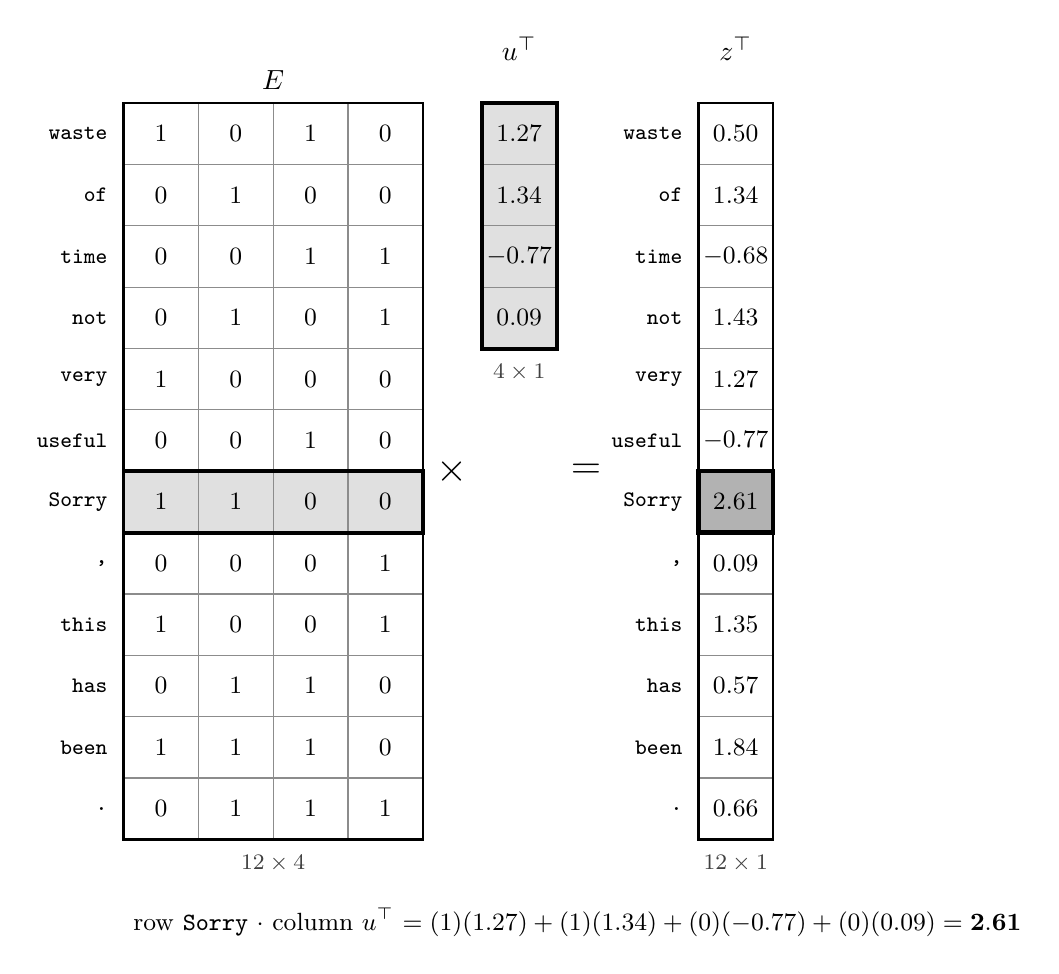
\begin{tikzpicture}
\draw[black!45, fill=white] (0.000,0.000) rectangle (0.950,-0.779);
\node[font=\small, text=black] at (0.475,-0.389) {$1$};
\draw[black!45, fill=white] (0.950,0.000) rectangle (1.900,-0.779);
\node[font=\small, text=black] at (1.425,-0.389) {$0$};
\draw[black!45, fill=white] (1.900,0.000) rectangle (2.850,-0.779);
\node[font=\small, text=black] at (2.375,-0.389) {$1$};
\draw[black!45, fill=white] (2.850,0.000) rectangle (3.800,-0.779);
\node[font=\small, text=black] at (3.325,-0.389) {$0$};
\draw[black!45, fill=white] (0.000,-0.779) rectangle (0.950,-1.558);
\node[font=\small, text=black] at (0.475,-1.168) {$0$};
\draw[black!45, fill=white] (0.950,-0.779) rectangle (1.900,-1.558);
\node[font=\small, text=black] at (1.425,-1.168) {$1$};
\draw[black!45, fill=white] (1.900,-0.779) rectangle (2.850,-1.558);
\node[font=\small, text=black] at (2.375,-1.168) {$0$};
\draw[black!45, fill=white] (2.850,-0.779) rectangle (3.800,-1.558);
\node[font=\small, text=black] at (3.325,-1.168) {$0$};
\draw[black!45, fill=white] (0.000,-1.558) rectangle (0.950,-2.337);
\node[font=\small, text=black] at (0.475,-1.947) {$0$};
\draw[black!45, fill=white] (0.950,-1.558) rectangle (1.900,-2.337);
\node[font=\small, text=black] at (1.425,-1.947) {$0$};
\draw[black!45, fill=white] (1.900,-1.558) rectangle (2.850,-2.337);
\node[font=\small, text=black] at (2.375,-1.947) {$1$};
\draw[black!45, fill=white] (2.850,-1.558) rectangle (3.800,-2.337);
\node[font=\small, text=black] at (3.325,-1.947) {$1$};
\draw[black!45, fill=white] (0.000,-2.337) rectangle (0.950,-3.116);
\node[font=\small, text=black] at (0.475,-2.726) {$0$};
\draw[black!45, fill=white] (0.950,-2.337) rectangle (1.900,-3.116);
\node[font=\small, text=black] at (1.425,-2.726) {$1$};
\draw[black!45, fill=white] (1.900,-2.337) rectangle (2.850,-3.116);
\node[font=\small, text=black] at (2.375,-2.726) {$0$};
\draw[black!45, fill=white] (2.850,-2.337) rectangle (3.800,-3.116);
\node[font=\small, text=black] at (3.325,-2.726) {$1$};
\draw[black!45, fill=white] (0.000,-3.116) rectangle (0.950,-3.895);
\node[font=\small, text=black] at (0.475,-3.505) {$1$};
\draw[black!45, fill=white] (0.950,-3.116) rectangle (1.900,-3.895);
\node[font=\small, text=black] at (1.425,-3.505) {$0$};
\draw[black!45, fill=white] (1.900,-3.116) rectangle (2.850,-3.895);
\node[font=\small, text=black] at (2.375,-3.505) {$0$};
\draw[black!45, fill=white] (2.850,-3.116) rectangle (3.800,-3.895);
\node[font=\small, text=black] at (3.325,-3.505) {$0$};
\draw[black!45, fill=white] (0.000,-3.895) rectangle (0.950,-4.674);
\node[font=\small, text=black] at (0.475,-4.284) {$0$};
\draw[black!45, fill=white] (0.950,-3.895) rectangle (1.900,-4.674);
\node[font=\small, text=black] at (1.425,-4.284) {$0$};
\draw[black!45, fill=white] (1.900,-3.895) rectangle (2.850,-4.674);
\node[font=\small, text=black] at (2.375,-4.284) {$1$};
\draw[black!45, fill=white] (2.850,-3.895) rectangle (3.800,-4.674);
\node[font=\small, text=black] at (3.325,-4.284) {$0$};
\draw[black!45, fill=black!12] (0.000,-4.674) rectangle (0.950,-5.453);
\node[font=\small, text=black] at (0.475,-5.063) {$1$};
\draw[black!45, fill=black!12] (0.950,-4.674) rectangle (1.900,-5.453);
\node[font=\small, text=black] at (1.425,-5.063) {$1$};
\draw[black!45, fill=black!12] (1.900,-4.674) rectangle (2.850,-5.453);
\node[font=\small, text=black] at (2.375,-5.063) {$0$};
\draw[black!45, fill=black!12] (2.850,-4.674) rectangle (3.800,-5.453);
\node[font=\small, text=black] at (3.325,-5.063) {$0$};
\draw[black!45, fill=white] (0.000,-5.453) rectangle (0.950,-6.232);
\node[font=\small, text=black] at (0.475,-5.842) {$0$};
\draw[black!45, fill=white] (0.950,-5.453) rectangle (1.900,-6.232);
\node[font=\small, text=black] at (1.425,-5.842) {$0$};
\draw[black!45, fill=white] (1.900,-5.453) rectangle (2.850,-6.232);
\node[font=\small, text=black] at (2.375,-5.842) {$0$};
\draw[black!45, fill=white] (2.850,-5.453) rectangle (3.800,-6.232);
\node[font=\small, text=black] at (3.325,-5.842) {$1$};
\draw[black!45, fill=white] (0.000,-6.232) rectangle (0.950,-7.011);
\node[font=\small, text=black] at (0.475,-6.621) {$1$};
\draw[black!45, fill=white] (0.950,-6.232) rectangle (1.900,-7.011);
\node[font=\small, text=black] at (1.425,-6.621) {$0$};
\draw[black!45, fill=white] (1.900,-6.232) rectangle (2.850,-7.011);
\node[font=\small, text=black] at (2.375,-6.621) {$0$};
\draw[black!45, fill=white] (2.850,-6.232) rectangle (3.800,-7.011);
\node[font=\small, text=black] at (3.325,-6.621) {$1$};
\draw[black!45, fill=white] (0.000,-7.011) rectangle (0.950,-7.790);
\node[font=\small, text=black] at (0.475,-7.400) {$0$};
\draw[black!45, fill=white] (0.950,-7.011) rectangle (1.900,-7.790);
\node[font=\small, text=black] at (1.425,-7.400) {$1$};
\draw[black!45, fill=white] (1.900,-7.011) rectangle (2.850,-7.790);
\node[font=\small, text=black] at (2.375,-7.400) {$1$};
\draw[black!45, fill=white] (2.850,-7.011) rectangle (3.800,-7.790);
\node[font=\small, text=black] at (3.325,-7.400) {$0$};
\draw[black!45, fill=white] (0.000,-7.790) rectangle (0.950,-8.569);
\node[font=\small, text=black] at (0.475,-8.179) {$1$};
\draw[black!45, fill=white] (0.950,-7.790) rectangle (1.900,-8.569);
\node[font=\small, text=black] at (1.425,-8.179) {$1$};
\draw[black!45, fill=white] (1.900,-7.790) rectangle (2.850,-8.569);
\node[font=\small, text=black] at (2.375,-8.179) {$1$};
\draw[black!45, fill=white] (2.850,-7.790) rectangle (3.800,-8.569);
\node[font=\small, text=black] at (3.325,-8.179) {$0$};
\draw[black!45, fill=white] (0.000,-8.569) rectangle (0.950,-9.348);
\node[font=\small, text=black] at (0.475,-8.958) {$0$};
\draw[black!45, fill=white] (0.950,-8.569) rectangle (1.900,-9.348);
\node[font=\small, text=black] at (1.425,-8.958) {$1$};
\draw[black!45, fill=white] (1.900,-8.569) rectangle (2.850,-9.348);
\node[font=\small, text=black] at (2.375,-8.958) {$1$};
\draw[black!45, fill=white] (2.850,-8.569) rectangle (3.800,-9.348);
\node[font=\small, text=black] at (3.325,-8.958) {$1$};
\draw[line width=1.4pt] (0.000,-4.674) rectangle (3.800,-5.453);
\draw[line width=0.9pt] (0.000,0.000) rectangle (3.800,-9.348);
\node[anchor=east, font=\footnotesize\ttfamily] at (-0.080,-0.389) {waste};
\node[anchor=east, font=\footnotesize\ttfamily] at (-0.080,-1.168) {of};
\node[anchor=east, font=\footnotesize\ttfamily] at (-0.080,-1.947) {time};
\node[anchor=east, font=\footnotesize\ttfamily] at (-0.080,-2.726) {not};
\node[anchor=east, font=\footnotesize\ttfamily] at (-0.080,-3.505) {very};
\node[anchor=east, font=\footnotesize\ttfamily] at (-0.080,-4.284) {useful};
\node[anchor=east, font=\footnotesize\ttfamily] at (-0.080,-5.063) {Sorry};
\node[anchor=east, font=\footnotesize\ttfamily] at (-0.080,-5.842) {{,}};
\node[anchor=east, font=\footnotesize\ttfamily] at (-0.080,-6.621) {this};
\node[anchor=east, font=\footnotesize\ttfamily] at (-0.080,-7.400) {has};
\node[anchor=east, font=\footnotesize\ttfamily] at (-0.080,-8.179) {been};
\node[anchor=east, font=\footnotesize\ttfamily] at (-0.080,-8.958) {.};
\node[anchor=south, font=\normalsize] at (1.900,0.050) {$E$};
\node[anchor=north, font=\footnotesize, text=black!75] at (1.900,-9.428) {$12\times4$};
\draw[black!45, fill=black!12] (4.550,0.000) rectangle (5.500,-0.779);
\node[font=\small, text=black] at (5.025,-0.389) {$1.27$};
\draw[black!45, fill=black!12] (4.550,-0.779) rectangle (5.500,-1.558);
\node[font=\small, text=black] at (5.025,-1.168) {$1.34$};
\draw[black!45, fill=black!12] (4.550,-1.558) rectangle (5.500,-2.337);
\node[font=\small, text=black] at (5.025,-1.947) {$-0.77$};
\draw[black!45, fill=black!12] (4.550,-2.337) rectangle (5.500,-3.116);
\node[font=\small, text=black] at (5.025,-2.726) {$0.09$};
\draw[line width=1.4pt] (4.550,0.000) rectangle (5.500,-3.116);
\draw[line width=0.9pt] (4.550,0.000) rectangle (5.500,-3.116);
\node[anchor=south, font=\normalsize] at (5.025,0.420) {$\bm{u}^\top$};
\node[anchor=north, font=\footnotesize, text=black!75] at (5.025,-3.196) {$4\times1$};
\draw[black!45, fill=white] (7.300,0.000) rectangle (8.250,-0.779);
\node[font=\small, text=black] at (7.775,-0.389) {$0.50$};
\draw[black!45, fill=white] (7.300,-0.779) rectangle (8.250,-1.558);
\node[font=\small, text=black] at (7.775,-1.168) {$1.34$};
\draw[black!45, fill=white] (7.300,-1.558) rectangle (8.250,-2.337);
\node[font=\small, text=black] at (7.775,-1.947) {$-0.68$};
\draw[black!45, fill=white] (7.300,-2.337) rectangle (8.250,-3.116);
\node[font=\small, text=black] at (7.775,-2.726) {$1.43$};
\draw[black!45, fill=white] (7.300,-3.116) rectangle (8.250,-3.895);
\node[font=\small, text=black] at (7.775,-3.505) {$1.27$};
\draw[black!45, fill=white] (7.300,-3.895) rectangle (8.250,-4.674);
\node[font=\small, text=black] at (7.775,-4.284) {$-0.77$};
\draw[black!45, fill=black!30] (7.300,-4.674) rectangle (8.250,-5.453);
\node[font=\small, text=black] at (7.775,-5.063) {$2.61$};
\draw[black!45, fill=white] (7.300,-5.453) rectangle (8.250,-6.232);
\node[font=\small, text=black] at (7.775,-5.842) {$0.09$};
\draw[black!45, fill=white] (7.300,-6.232) rectangle (8.250,-7.011);
\node[font=\small, text=black] at (7.775,-6.621) {$1.35$};
\draw[black!45, fill=white] (7.300,-7.011) rectangle (8.250,-7.790);
\node[font=\small, text=black] at (7.775,-7.400) {$0.57$};
\draw[black!45, fill=white] (7.300,-7.790) rectangle (8.250,-8.569);
\node[font=\small, text=black] at (7.775,-8.179) {$1.84$};
\draw[black!45, fill=white] (7.300,-8.569) rectangle (8.250,-9.348);
\node[font=\small, text=black] at (7.775,-8.958) {$0.66$};
\draw[line width=1.6pt] (7.300,-4.674) rectangle (8.250,-5.453);
\draw[line width=0.9pt] (7.300,0.000) rectangle (8.250,-9.348);
\node[anchor=east, font=\footnotesize\ttfamily] at (7.220,-0.389) {waste};
\node[anchor=east, font=\footnotesize\ttfamily] at (7.220,-1.168) {of};
\node[anchor=east, font=\footnotesize\ttfamily] at (7.220,-1.947) {time};
\node[anchor=east, font=\footnotesize\ttfamily] at (7.220,-2.726) {not};
\node[anchor=east, font=\footnotesize\ttfamily] at (7.220,-3.505) {very};
\node[anchor=east, font=\footnotesize\ttfamily] at (7.220,-4.284) {useful};
\node[anchor=east, font=\footnotesize\ttfamily] at (7.220,-5.063) {Sorry};
\node[anchor=east, font=\footnotesize\ttfamily] at (7.220,-5.842) {{,}};
\node[anchor=east, font=\footnotesize\ttfamily] at (7.220,-6.621) {this};
\node[anchor=east, font=\footnotesize\ttfamily] at (7.220,-7.400) {has};
\node[anchor=east, font=\footnotesize\ttfamily] at (7.220,-8.179) {been};
\node[anchor=east, font=\footnotesize\ttfamily] at (7.220,-8.958) {.};
\node[anchor=south, font=\normalsize] at (7.775,0.420) {$\bm{z}^\top$};
\node[anchor=north, font=\footnotesize, text=black!75] at (7.775,-9.428) {$12\times1$};
\node[font=\Large] at (4.175,-4.674) {$\times$};
\node[font=\Large] at (5.875,-4.674) {$=$};
\node[anchor=north west, font=\small, align=left] at (0,-10.098) {row \texttt{Sorry} $\cdot$ column $\bm{u}^\top$ $= (1)(1.27) + (1)(1.34) + (0)(-0.77) + (0)(0.09) = \mathbf{2.61}$};
\end{tikzpicture}

\captionof{figure}{Scoring every word. The highlighted row is \tok{Sorry}'s arrow; it meets the column $\bm{u}^\top$, and
the dot product, written out underneath, is \tok{Sorry}'s logit. Every other row does the same with its own
arrow.}\label{fig:ch7scores}
\end{minipage}\par\medskip

For a whole batch, the shape is $B\times T\times V$: one score per word, per position, per sentence, the end of
the road in Chapter 1, \S1.9. Here are both customer replies of Chapter 3 at once:

\par\medskip\noindent\begin{minipage}{\linewidth}\centering
% AUTO-GENERATED by code/ch7_figs.py
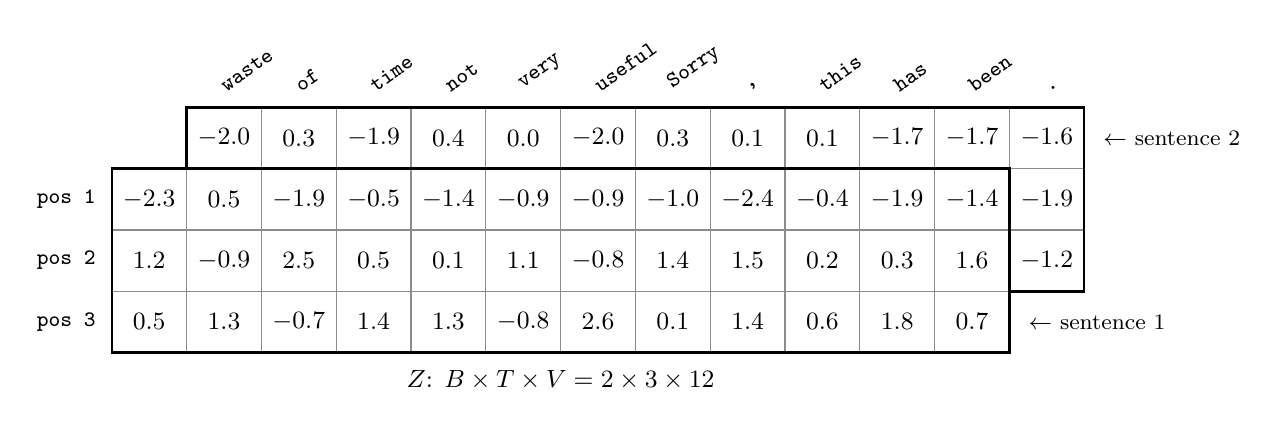
\begin{tikzpicture}
\fill[white] (0.950,0.779) rectangle (12.350,-1.558);
\draw[black!45, fill=white] (0.950,0.779) rectangle (1.900,0.000);
\node[font=\small, text=black] at (1.425,0.389) {$-2.0$};
\draw[black!45, fill=white] (1.900,0.779) rectangle (2.850,0.000);
\node[font=\small, text=black] at (2.375,0.389) {$0.3$};
\draw[black!45, fill=white] (2.850,0.779) rectangle (3.800,0.000);
\node[font=\small, text=black] at (3.325,0.389) {$-1.9$};
\draw[black!45, fill=white] (3.800,0.779) rectangle (4.750,0.000);
\node[font=\small, text=black] at (4.275,0.389) {$0.4$};
\draw[black!45, fill=white] (4.750,0.779) rectangle (5.700,0.000);
\node[font=\small, text=black] at (5.225,0.389) {$0.0$};
\draw[black!45, fill=white] (5.700,0.779) rectangle (6.650,0.000);
\node[font=\small, text=black] at (6.175,0.389) {$-2.0$};
\draw[black!45, fill=white] (6.650,0.779) rectangle (7.600,0.000);
\node[font=\small, text=black] at (7.125,0.389) {$0.3$};
\draw[black!45, fill=white] (7.600,0.779) rectangle (8.550,0.000);
\node[font=\small, text=black] at (8.075,0.389) {$0.1$};
\draw[black!45, fill=white] (8.550,0.779) rectangle (9.500,0.000);
\node[font=\small, text=black] at (9.025,0.389) {$0.1$};
\draw[black!45, fill=white] (9.500,0.779) rectangle (10.450,0.000);
\node[font=\small, text=black] at (9.975,0.389) {$-1.7$};
\draw[black!45, fill=white] (10.450,0.779) rectangle (11.400,0.000);
\node[font=\small, text=black] at (10.925,0.389) {$-1.7$};
\draw[black!45, fill=white] (11.400,0.779) rectangle (12.350,0.000);
\node[font=\small, text=black] at (11.875,0.389) {$-1.6$};
\draw[black!45, fill=white] (0.950,0.000) rectangle (1.900,-0.779);
\node[font=\small, text=black] at (1.425,-0.389) {$-2.6$};
\draw[black!45, fill=white] (1.900,0.000) rectangle (2.850,-0.779);
\node[font=\small, text=black] at (2.375,-0.389) {$-0.7$};
\draw[black!45, fill=white] (2.850,0.000) rectangle (3.800,-0.779);
\node[font=\small, text=black] at (3.325,-0.389) {$-1.2$};
\draw[black!45, fill=white] (3.800,0.000) rectangle (4.750,-0.779);
\node[font=\small, text=black] at (4.275,-0.389) {$-1.0$};
\draw[black!45, fill=white] (4.750,0.000) rectangle (5.700,-0.779);
\node[font=\small, text=black] at (5.225,-0.389) {$-1.6$};
\draw[black!45, fill=white] (5.700,0.000) rectangle (6.650,-0.779);
\node[font=\small, text=black] at (6.175,-0.389) {$-1.0$};
\draw[black!45, fill=white] (6.650,0.000) rectangle (7.600,-0.779);
\node[font=\small, text=black] at (7.125,-0.389) {$-2.3$};
\draw[black!45, fill=white] (7.600,0.000) rectangle (8.550,-0.779);
\node[font=\small, text=black] at (8.075,-0.389) {$-0.3$};
\draw[black!45, fill=white] (8.550,0.000) rectangle (9.500,-0.779);
\node[font=\small, text=black] at (9.025,-0.389) {$-1.9$};
\draw[black!45, fill=white] (9.500,0.000) rectangle (10.450,-0.779);
\node[font=\small, text=black] at (9.975,-0.389) {$-1.7$};
\draw[black!45, fill=white] (10.450,0.000) rectangle (11.400,-0.779);
\node[font=\small, text=black] at (10.925,-0.389) {$-3.2$};
\draw[black!45, fill=white] (11.400,0.000) rectangle (12.350,-0.779);
\node[font=\small, text=black] at (11.875,-0.389) {$-1.9$};
\draw[black!45, fill=white] (0.950,-0.779) rectangle (1.900,-1.558);
\node[font=\small, text=black] at (1.425,-1.168) {$-1.2$};
\draw[black!45, fill=white] (1.900,-0.779) rectangle (2.850,-1.558);
\node[font=\small, text=black] at (2.375,-1.168) {$0.6$};
\draw[black!45, fill=white] (2.850,-0.779) rectangle (3.800,-1.558);
\node[font=\small, text=black] at (3.325,-1.168) {$-1.8$};
\draw[black!45, fill=white] (3.800,-0.779) rectangle (4.750,-1.558);
\node[font=\small, text=black] at (4.275,-1.168) {$0.7$};
\draw[black!45, fill=white] (4.750,-0.779) rectangle (5.700,-1.558);
\node[font=\small, text=black] at (5.225,-1.168) {$0.6$};
\draw[black!45, fill=white] (5.700,-0.779) rectangle (6.650,-1.558);
\node[font=\small, text=black] at (6.175,-1.168) {$-1.8$};
\draw[black!45, fill=white] (6.650,-0.779) rectangle (7.600,-1.558);
\node[font=\small, text=black] at (7.125,-1.168) {$1.2$};
\draw[black!45, fill=white] (7.600,-0.779) rectangle (8.550,-1.558);
\node[font=\small, text=black] at (8.075,-1.168) {$0.0$};
\draw[black!45, fill=white] (8.550,-0.779) rectangle (9.500,-1.558);
\node[font=\small, text=black] at (9.025,-1.168) {$0.7$};
\draw[black!45, fill=white] (9.500,-0.779) rectangle (10.450,-1.558);
\node[font=\small, text=black] at (9.975,-1.168) {$-1.2$};
\draw[black!45, fill=white] (10.450,-0.779) rectangle (11.400,-1.558);
\node[font=\small, text=black] at (10.925,-1.168) {$-0.6$};
\draw[black!45, fill=white] (11.400,-0.779) rectangle (12.350,-1.558);
\node[font=\small, text=black] at (11.875,-1.168) {$-1.2$};
\draw[line width=0.9pt] (0.950,0.779) rectangle (12.350,-1.558);
\node[anchor=south west, rotate=35, font=\footnotesize\ttfamily] at (1.425,0.799) {waste};
\node[anchor=south west, rotate=35, font=\footnotesize\ttfamily] at (2.375,0.799) {of};
\node[anchor=south west, rotate=35, font=\footnotesize\ttfamily] at (3.325,0.799) {time};
\node[anchor=south west, rotate=35, font=\footnotesize\ttfamily] at (4.275,0.799) {not};
\node[anchor=south west, rotate=35, font=\footnotesize\ttfamily] at (5.225,0.799) {very};
\node[anchor=south west, rotate=35, font=\footnotesize\ttfamily] at (6.175,0.799) {useful};
\node[anchor=south west, rotate=35, font=\footnotesize\ttfamily] at (7.125,0.799) {Sorry};
\node[anchor=south west, rotate=35, font=\footnotesize\ttfamily] at (8.075,0.799) {{,}};
\node[anchor=south west, rotate=35, font=\footnotesize\ttfamily] at (9.025,0.799) {this};
\node[anchor=south west, rotate=35, font=\footnotesize\ttfamily] at (9.975,0.799) {has};
\node[anchor=south west, rotate=35, font=\footnotesize\ttfamily] at (10.925,0.799) {been};
\node[anchor=south west, rotate=35, font=\footnotesize\ttfamily] at (11.875,0.799) {.};
\node[anchor=west, font=\footnotesize] at (12.470,0.389) {$\leftarrow$ sentence 2};
\fill[white] (0.000,0.000) rectangle (11.400,-2.337);
\draw[black!45, fill=white] (0.000,0.000) rectangle (0.950,-0.779);
\node[font=\small, text=black] at (0.475,-0.389) {$-2.3$};
\draw[black!45, fill=white] (0.950,0.000) rectangle (1.900,-0.779);
\node[font=\small, text=black] at (1.425,-0.389) {$0.5$};
\draw[black!45, fill=white] (1.900,0.000) rectangle (2.850,-0.779);
\node[font=\small, text=black] at (2.375,-0.389) {$-1.9$};
\draw[black!45, fill=white] (2.850,0.000) rectangle (3.800,-0.779);
\node[font=\small, text=black] at (3.325,-0.389) {$-0.5$};
\draw[black!45, fill=white] (3.800,0.000) rectangle (4.750,-0.779);
\node[font=\small, text=black] at (4.275,-0.389) {$-1.4$};
\draw[black!45, fill=white] (4.750,0.000) rectangle (5.700,-0.779);
\node[font=\small, text=black] at (5.225,-0.389) {$-0.9$};
\draw[black!45, fill=white] (5.700,0.000) rectangle (6.650,-0.779);
\node[font=\small, text=black] at (6.175,-0.389) {$-0.9$};
\draw[black!45, fill=white] (6.650,0.000) rectangle (7.600,-0.779);
\node[font=\small, text=black] at (7.125,-0.389) {$-1.0$};
\draw[black!45, fill=white] (7.600,0.000) rectangle (8.550,-0.779);
\node[font=\small, text=black] at (8.075,-0.389) {$-2.4$};
\draw[black!45, fill=white] (8.550,0.000) rectangle (9.500,-0.779);
\node[font=\small, text=black] at (9.025,-0.389) {$-0.4$};
\draw[black!45, fill=white] (9.500,0.000) rectangle (10.450,-0.779);
\node[font=\small, text=black] at (9.975,-0.389) {$-1.9$};
\draw[black!45, fill=white] (10.450,0.000) rectangle (11.400,-0.779);
\node[font=\small, text=black] at (10.925,-0.389) {$-1.4$};
\draw[black!45, fill=white] (0.000,-0.779) rectangle (0.950,-1.558);
\node[font=\small, text=black] at (0.475,-1.168) {$1.2$};
\draw[black!45, fill=white] (0.950,-0.779) rectangle (1.900,-1.558);
\node[font=\small, text=black] at (1.425,-1.168) {$-0.9$};
\draw[black!45, fill=white] (1.900,-0.779) rectangle (2.850,-1.558);
\node[font=\small, text=black] at (2.375,-1.168) {$2.5$};
\draw[black!45, fill=white] (2.850,-0.779) rectangle (3.800,-1.558);
\node[font=\small, text=black] at (3.325,-1.168) {$0.5$};
\draw[black!45, fill=white] (3.800,-0.779) rectangle (4.750,-1.558);
\node[font=\small, text=black] at (4.275,-1.168) {$0.1$};
\draw[black!45, fill=white] (4.750,-0.779) rectangle (5.700,-1.558);
\node[font=\small, text=black] at (5.225,-1.168) {$1.1$};
\draw[black!45, fill=white] (5.700,-0.779) rectangle (6.650,-1.558);
\node[font=\small, text=black] at (6.175,-1.168) {$-0.8$};
\draw[black!45, fill=white] (6.650,-0.779) rectangle (7.600,-1.558);
\node[font=\small, text=black] at (7.125,-1.168) {$1.4$};
\draw[black!45, fill=white] (7.600,-0.779) rectangle (8.550,-1.558);
\node[font=\small, text=black] at (8.075,-1.168) {$1.5$};
\draw[black!45, fill=white] (8.550,-0.779) rectangle (9.500,-1.558);
\node[font=\small, text=black] at (9.025,-1.168) {$0.2$};
\draw[black!45, fill=white] (9.500,-0.779) rectangle (10.450,-1.558);
\node[font=\small, text=black] at (9.975,-1.168) {$0.3$};
\draw[black!45, fill=white] (10.450,-0.779) rectangle (11.400,-1.558);
\node[font=\small, text=black] at (10.925,-1.168) {$1.6$};
\draw[black!45, fill=white] (0.000,-1.558) rectangle (0.950,-2.337);
\node[font=\small, text=black] at (0.475,-1.947) {$0.5$};
\draw[black!45, fill=white] (0.950,-1.558) rectangle (1.900,-2.337);
\node[font=\small, text=black] at (1.425,-1.947) {$1.3$};
\draw[black!45, fill=white] (1.900,-1.558) rectangle (2.850,-2.337);
\node[font=\small, text=black] at (2.375,-1.947) {$-0.7$};
\draw[black!45, fill=white] (2.850,-1.558) rectangle (3.800,-2.337);
\node[font=\small, text=black] at (3.325,-1.947) {$1.4$};
\draw[black!45, fill=white] (3.800,-1.558) rectangle (4.750,-2.337);
\node[font=\small, text=black] at (4.275,-1.947) {$1.3$};
\draw[black!45, fill=white] (4.750,-1.558) rectangle (5.700,-2.337);
\node[font=\small, text=black] at (5.225,-1.947) {$-0.8$};
\draw[black!45, fill=white] (5.700,-1.558) rectangle (6.650,-2.337);
\node[font=\small, text=black] at (6.175,-1.947) {$2.6$};
\draw[black!45, fill=white] (6.650,-1.558) rectangle (7.600,-2.337);
\node[font=\small, text=black] at (7.125,-1.947) {$0.1$};
\draw[black!45, fill=white] (7.600,-1.558) rectangle (8.550,-2.337);
\node[font=\small, text=black] at (8.075,-1.947) {$1.4$};
\draw[black!45, fill=white] (8.550,-1.558) rectangle (9.500,-2.337);
\node[font=\small, text=black] at (9.025,-1.947) {$0.6$};
\draw[black!45, fill=white] (9.500,-1.558) rectangle (10.450,-2.337);
\node[font=\small, text=black] at (9.975,-1.947) {$1.8$};
\draw[black!45, fill=white] (10.450,-1.558) rectangle (11.400,-2.337);
\node[font=\small, text=black] at (10.925,-1.947) {$0.7$};
\draw[line width=0.9pt] (0.000,0.000) rectangle (11.400,-2.337);
\node[anchor=east, font=\footnotesize\ttfamily] at (-0.080,-0.389) {pos 1};
\node[anchor=east, font=\footnotesize\ttfamily] at (-0.080,-1.168) {pos 2};
\node[anchor=east, font=\footnotesize\ttfamily] at (-0.080,-1.947) {pos 3};
\node[anchor=west, font=\footnotesize] at (11.520,-1.947) {$\leftarrow$ sentence 1};
\node[anchor=north, font=\small] at (5.700,-2.437) {$Z$: $B\times T\times V = 2\times3\times12$};
\end{tikzpicture}

\captionof{figure}{Logits for a batch of $B=2$ sentences of $T=3$ tokens over $V=12$ words. Each row is one position's
twelve scores; the word labels sit on the back sheet, and the front sheet's columns are the same twelve words. The
front sheet is \tok{waste of time}; its third row is the column in the figure above.}
\end{minipage}\par\medskip
 Our toy reuses the input table $E$ at
the output. This \emph{tying} saves a $d\times V$ matrix, and GPT-2 does the same (Press and Wolf, 2017). Other
models learn a separate output matrix, often written $W_{\text{vocab}}$.

Each score is length times length times agreement (Chapter 3, \S3.2). Here is every word, sorted by score:

\begin{center}
\small
\begin{tabular}{@{}l c c c r r r@{}}
\toprule
word & arrow $\bm{e}_w$ & $\lVert\bm{e}_w\rVert$ & angle to $\bm{u}$ & logit $\bm{u}\cdot\bm{e}_w$ & $e^{\text{logit}}$ & probability\\
\midrule
\csname @@input\endcsname data_ch7/logit_rows.tex
\bottomrule
\end{tabular}
\end{center}

\tok{Sorry} wins: its arrow is only \nSevenAngSorry$^\circ$ from $\bm{u}$. Now look at \tok{of} and \tok{been}.
\tok{of} points closer to $\bm{u}$ (\nSevenAngOf$^\circ$) than \tok{been} does (\nSevenAngBeen$^\circ$), yet \tok{been}
scores higher, \nSevenLogitBeen\ against \nSevenLogitOf. The reason is the other knob: \tok{been}'s arrow has
length \nSevenLenBeen, \tok{of}'s only \nSevenLenOf. Direction and length both count.

\begin{breaks}
Signposts are fixed in the ground. Here the ``signposts'' are the same arrows the model reads at its input, and
they are learned: training moves them so that the right word's signpost ends up pointing where the model's needle
points.
\end{breaks}

\Why Why compare with the embedding table and not with something new? The output must be one of the $V$ tokens the
model knows, and the embedding table already holds one arrow per token. Scoring by dot product reuses the
geometry of every earlier chapter: agreement times length.

\begin{wrongidea}{7.1}
\emph{The model can write any word, even one it has never seen.} The last step scores exactly $V$ tokens, no more.
It is tempting because the text that comes out looks free. But the output layer has one row per vocabulary entry
and nothing else, so the next token is always one of those $V$. New words still appear in its writing, but as sequences of known pieces (Chapter 2).
\end{wrongidea}

\begin{checkq}
A model has a vocabulary of $V$ tokens and width $d$. One pass over a batch of $B$ sentences of $T$ tokens
produces logits of what shape?
\begin{options}
\item $B\times T\times d$, one arrow per position.
\item $B\times T\times V$, one score per word per position.
\item $B\times V$, one score per word per sentence, for the last position only.
\item $B\times T\times (V+1)$, with an extra slot for new words.
\end{options}
\end{checkq}

\Summary{The final arrow is scored against every token's arrow by dot product, giving one logit per word.}

%---------------------------------------------------------------------
\subsection*{7.2\quad From scores to probabilities}

The logits can be negative and do not add to 1. We turn them into shares with the same softmax as Chapter 3,
now over all $V=\nSevenV$ words instead of three tokens:
\[
P(w) = \frac{e^{z_w}}{\sum_{w'} e^{z_{w'}}} \shape{1\times V\ \to\ 1\times V}
\]
As vectors, one line per step:

\par\medskip\noindent\begin{minipage}{\linewidth}\centering
% AUTO-GENERATED by code/ch7_figs.py
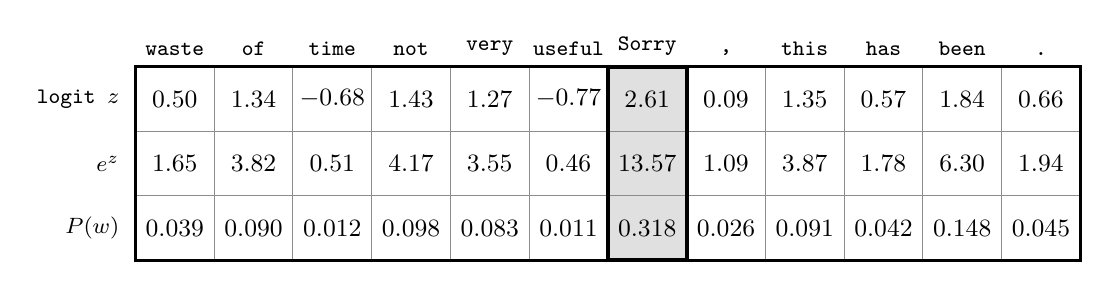
\begin{tikzpicture}
\draw[black!45, fill=white] (0.000,0.000) rectangle (1.000,-0.820);
\node[font=\small, text=black] at (0.500,-0.410) {$0.50$};
\draw[black!45, fill=white] (1.000,0.000) rectangle (2.000,-0.820);
\node[font=\small, text=black] at (1.500,-0.410) {$1.34$};
\draw[black!45, fill=white] (2.000,0.000) rectangle (3.000,-0.820);
\node[font=\small, text=black] at (2.500,-0.410) {$-0.68$};
\draw[black!45, fill=white] (3.000,0.000) rectangle (4.000,-0.820);
\node[font=\small, text=black] at (3.500,-0.410) {$1.43$};
\draw[black!45, fill=white] (4.000,0.000) rectangle (5.000,-0.820);
\node[font=\small, text=black] at (4.500,-0.410) {$1.27$};
\draw[black!45, fill=white] (5.000,0.000) rectangle (6.000,-0.820);
\node[font=\small, text=black] at (5.500,-0.410) {$-0.77$};
\draw[black!45, fill=black!12] (6.000,0.000) rectangle (7.000,-0.820);
\node[font=\small, text=black] at (6.500,-0.410) {$2.61$};
\draw[black!45, fill=white] (7.000,0.000) rectangle (8.000,-0.820);
\node[font=\small, text=black] at (7.500,-0.410) {$0.09$};
\draw[black!45, fill=white] (8.000,0.000) rectangle (9.000,-0.820);
\node[font=\small, text=black] at (8.500,-0.410) {$1.35$};
\draw[black!45, fill=white] (9.000,0.000) rectangle (10.000,-0.820);
\node[font=\small, text=black] at (9.500,-0.410) {$0.57$};
\draw[black!45, fill=white] (10.000,0.000) rectangle (11.000,-0.820);
\node[font=\small, text=black] at (10.500,-0.410) {$1.84$};
\draw[black!45, fill=white] (11.000,0.000) rectangle (12.000,-0.820);
\node[font=\small, text=black] at (11.500,-0.410) {$0.66$};
\draw[black!45, fill=white] (0.000,-0.820) rectangle (1.000,-1.640);
\node[font=\small, text=black] at (0.500,-1.230) {$1.65$};
\draw[black!45, fill=white] (1.000,-0.820) rectangle (2.000,-1.640);
\node[font=\small, text=black] at (1.500,-1.230) {$3.82$};
\draw[black!45, fill=white] (2.000,-0.820) rectangle (3.000,-1.640);
\node[font=\small, text=black] at (2.500,-1.230) {$0.51$};
\draw[black!45, fill=white] (3.000,-0.820) rectangle (4.000,-1.640);
\node[font=\small, text=black] at (3.500,-1.230) {$4.17$};
\draw[black!45, fill=white] (4.000,-0.820) rectangle (5.000,-1.640);
\node[font=\small, text=black] at (4.500,-1.230) {$3.55$};
\draw[black!45, fill=white] (5.000,-0.820) rectangle (6.000,-1.640);
\node[font=\small, text=black] at (5.500,-1.230) {$0.46$};
\draw[black!45, fill=black!12] (6.000,-0.820) rectangle (7.000,-1.640);
\node[font=\small, text=black] at (6.500,-1.230) {$13.57$};
\draw[black!45, fill=white] (7.000,-0.820) rectangle (8.000,-1.640);
\node[font=\small, text=black] at (7.500,-1.230) {$1.09$};
\draw[black!45, fill=white] (8.000,-0.820) rectangle (9.000,-1.640);
\node[font=\small, text=black] at (8.500,-1.230) {$3.87$};
\draw[black!45, fill=white] (9.000,-0.820) rectangle (10.000,-1.640);
\node[font=\small, text=black] at (9.500,-1.230) {$1.78$};
\draw[black!45, fill=white] (10.000,-0.820) rectangle (11.000,-1.640);
\node[font=\small, text=black] at (10.500,-1.230) {$6.30$};
\draw[black!45, fill=white] (11.000,-0.820) rectangle (12.000,-1.640);
\node[font=\small, text=black] at (11.500,-1.230) {$1.94$};
\draw[black!45, fill=white] (0.000,-1.640) rectangle (1.000,-2.460);
\node[font=\small, text=black] at (0.500,-2.050) {$0.039$};
\draw[black!45, fill=white] (1.000,-1.640) rectangle (2.000,-2.460);
\node[font=\small, text=black] at (1.500,-2.050) {$0.090$};
\draw[black!45, fill=white] (2.000,-1.640) rectangle (3.000,-2.460);
\node[font=\small, text=black] at (2.500,-2.050) {$0.012$};
\draw[black!45, fill=white] (3.000,-1.640) rectangle (4.000,-2.460);
\node[font=\small, text=black] at (3.500,-2.050) {$0.098$};
\draw[black!45, fill=white] (4.000,-1.640) rectangle (5.000,-2.460);
\node[font=\small, text=black] at (4.500,-2.050) {$0.083$};
\draw[black!45, fill=white] (5.000,-1.640) rectangle (6.000,-2.460);
\node[font=\small, text=black] at (5.500,-2.050) {$0.011$};
\draw[black!45, fill=black!12] (6.000,-1.640) rectangle (7.000,-2.460);
\node[font=\small, text=black] at (6.500,-2.050) {$0.318$};
\draw[black!45, fill=white] (7.000,-1.640) rectangle (8.000,-2.460);
\node[font=\small, text=black] at (7.500,-2.050) {$0.026$};
\draw[black!45, fill=white] (8.000,-1.640) rectangle (9.000,-2.460);
\node[font=\small, text=black] at (8.500,-2.050) {$0.091$};
\draw[black!45, fill=white] (9.000,-1.640) rectangle (10.000,-2.460);
\node[font=\small, text=black] at (9.500,-2.050) {$0.042$};
\draw[black!45, fill=white] (10.000,-1.640) rectangle (11.000,-2.460);
\node[font=\small, text=black] at (10.500,-2.050) {$0.148$};
\draw[black!45, fill=white] (11.000,-1.640) rectangle (12.000,-2.460);
\node[font=\small, text=black] at (11.500,-2.050) {$0.045$};
\draw[line width=1.4pt] (6.000,0.000) rectangle (7.000,-2.460);
\draw[line width=0.9pt] (0.000,0.000) rectangle (12.000,-2.460);
\node[anchor=east, font=\footnotesize\ttfamily] at (-0.080,-0.410) {logit $z$};
\node[anchor=east, font=\footnotesize\ttfamily] at (-0.080,-1.230) {$e^{z}$};
\node[anchor=east, font=\footnotesize\ttfamily] at (-0.080,-2.050) {$P(w)$};
\node[anchor=south, font=\footnotesize\ttfamily] at (0.500,0.020) {waste};
\node[anchor=south, font=\footnotesize\ttfamily] at (1.500,0.020) {of};
\node[anchor=south, font=\footnotesize\ttfamily] at (2.500,0.020) {time};
\node[anchor=south, font=\footnotesize\ttfamily] at (3.500,0.020) {not};
\node[anchor=south, font=\footnotesize\ttfamily] at (4.500,0.020) {very};
\node[anchor=south, font=\footnotesize\ttfamily] at (5.500,0.020) {useful};
\node[anchor=south, font=\footnotesize\ttfamily] at (6.500,0.020) {Sorry};
\node[anchor=south, font=\footnotesize\ttfamily] at (7.500,0.020) {{,}};
\node[anchor=south, font=\footnotesize\ttfamily] at (8.500,0.020) {this};
\node[anchor=south, font=\footnotesize\ttfamily] at (9.500,0.020) {has};
\node[anchor=south, font=\footnotesize\ttfamily] at (10.500,0.020) {been};
\node[anchor=south, font=\footnotesize\ttfamily] at (11.500,0.020) {.};
\end{tikzpicture}

\captionof{figure}{Softmax on the twelve logits of \tok{time}. Top: logits. Middle: $e$ to each logit, all positive.
Bottom: each middle number divided by their total; the bottom line adds to 1. \tok{Sorry}'s column is
highlighted.}
\end{minipage}\par\medskip

For our arrow, the total of the $e^{\text{logit}}$ line is \nSevenExpSum, and \tok{Sorry} gets
$P=\nSevenPSorry$, against $\nSevenUniform$ if all twelve words were equally likely. \tok{\nSevenSecond} comes
second with \nSevenPBeen.

\Sanity The probabilities in the table add to 1, and \tok{Sorry} has the largest logit and the largest
probability. One more check you can do in your head: the ratio of two probabilities depends only on the gap
between their logits. The gap between \tok{Sorry} and \tok{\nSevenSecond} is \nSevenGap, and
$e^{\nSevenGap}\approx\nSevenOdds$, which matches $\nSevenPSorry/\nSevenPBeen\approx\nSevenOddsCheck$.

\Why Softmax keeps the three properties that Chapter 3 asked for: positive shares, only differences matter, and
leaders lead. A logit is ``how much more than the others'', and softmax turns ``how much more'' into ``how
often''.

\Summary{Softmax turns the logits into one probability per word, and only the gaps between logits matter.}

%---------------------------------------------------------------------
\subsection*{7.3\quad Temperature: how bold to be}

\Predict Divide every logit by 2 before the softmax. Will \tok{Sorry}'s probability go up or down? What if you
divide by 0.5?

\Picture A dimmer switch on how decisive the model is. Turned down, the favourite takes nearly everything. Turned
up, the long shots get a real chance. In Chapter 3 you met the same knob as the \emph{length} of a query: a longer
query gave a more decisive softmax. Dividing logits by a temperature $\tau$ shrinks or stretches all the gaps at
once.

\Exactly $P_\tau(w)=\dfrac{e^{z_w/\tau}}{\sum_{w'} e^{z_{w'}/\tau}}$. Here is the whole probability vector at
three temperatures:

\par\medskip\noindent\begin{minipage}{\linewidth}\centering
% AUTO-GENERATED by code/ch7_figs.py
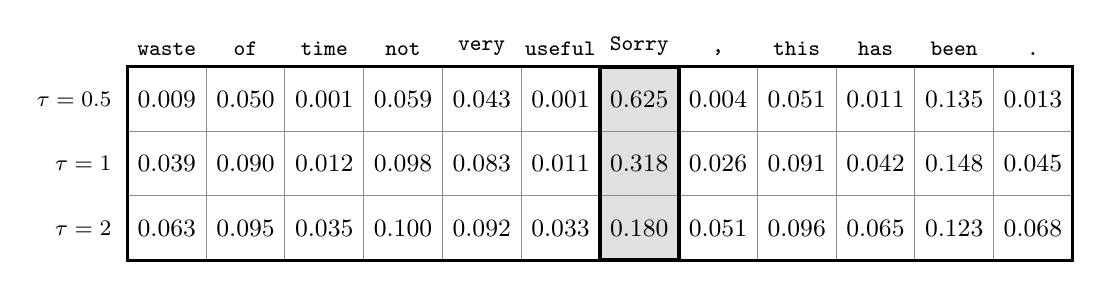
\begin{tikzpicture}
\draw[black!45, fill=white] (0.000,0.000) rectangle (1.000,-0.820);
\node[font=\small, text=black] at (0.500,-0.410) {$0.009$};
\draw[black!45, fill=white] (1.000,0.000) rectangle (2.000,-0.820);
\node[font=\small, text=black] at (1.500,-0.410) {$0.050$};
\draw[black!45, fill=white] (2.000,0.000) rectangle (3.000,-0.820);
\node[font=\small, text=black] at (2.500,-0.410) {$0.001$};
\draw[black!45, fill=white] (3.000,0.000) rectangle (4.000,-0.820);
\node[font=\small, text=black] at (3.500,-0.410) {$0.059$};
\draw[black!45, fill=white] (4.000,0.000) rectangle (5.000,-0.820);
\node[font=\small, text=black] at (4.500,-0.410) {$0.043$};
\draw[black!45, fill=white] (5.000,0.000) rectangle (6.000,-0.820);
\node[font=\small, text=black] at (5.500,-0.410) {$0.001$};
\draw[black!45, fill=black!12] (6.000,0.000) rectangle (7.000,-0.820);
\node[font=\small, text=black] at (6.500,-0.410) {$0.625$};
\draw[black!45, fill=white] (7.000,0.000) rectangle (8.000,-0.820);
\node[font=\small, text=black] at (7.500,-0.410) {$0.004$};
\draw[black!45, fill=white] (8.000,0.000) rectangle (9.000,-0.820);
\node[font=\small, text=black] at (8.500,-0.410) {$0.051$};
\draw[black!45, fill=white] (9.000,0.000) rectangle (10.000,-0.820);
\node[font=\small, text=black] at (9.500,-0.410) {$0.011$};
\draw[black!45, fill=white] (10.000,0.000) rectangle (11.000,-0.820);
\node[font=\small, text=black] at (10.500,-0.410) {$0.135$};
\draw[black!45, fill=white] (11.000,0.000) rectangle (12.000,-0.820);
\node[font=\small, text=black] at (11.500,-0.410) {$0.013$};
\draw[black!45, fill=white] (0.000,-0.820) rectangle (1.000,-1.640);
\node[font=\small, text=black] at (0.500,-1.230) {$0.039$};
\draw[black!45, fill=white] (1.000,-0.820) rectangle (2.000,-1.640);
\node[font=\small, text=black] at (1.500,-1.230) {$0.090$};
\draw[black!45, fill=white] (2.000,-0.820) rectangle (3.000,-1.640);
\node[font=\small, text=black] at (2.500,-1.230) {$0.012$};
\draw[black!45, fill=white] (3.000,-0.820) rectangle (4.000,-1.640);
\node[font=\small, text=black] at (3.500,-1.230) {$0.098$};
\draw[black!45, fill=white] (4.000,-0.820) rectangle (5.000,-1.640);
\node[font=\small, text=black] at (4.500,-1.230) {$0.083$};
\draw[black!45, fill=white] (5.000,-0.820) rectangle (6.000,-1.640);
\node[font=\small, text=black] at (5.500,-1.230) {$0.011$};
\draw[black!45, fill=black!12] (6.000,-0.820) rectangle (7.000,-1.640);
\node[font=\small, text=black] at (6.500,-1.230) {$0.318$};
\draw[black!45, fill=white] (7.000,-0.820) rectangle (8.000,-1.640);
\node[font=\small, text=black] at (7.500,-1.230) {$0.026$};
\draw[black!45, fill=white] (8.000,-0.820) rectangle (9.000,-1.640);
\node[font=\small, text=black] at (8.500,-1.230) {$0.091$};
\draw[black!45, fill=white] (9.000,-0.820) rectangle (10.000,-1.640);
\node[font=\small, text=black] at (9.500,-1.230) {$0.042$};
\draw[black!45, fill=white] (10.000,-0.820) rectangle (11.000,-1.640);
\node[font=\small, text=black] at (10.500,-1.230) {$0.148$};
\draw[black!45, fill=white] (11.000,-0.820) rectangle (12.000,-1.640);
\node[font=\small, text=black] at (11.500,-1.230) {$0.045$};
\draw[black!45, fill=white] (0.000,-1.640) rectangle (1.000,-2.460);
\node[font=\small, text=black] at (0.500,-2.050) {$0.063$};
\draw[black!45, fill=white] (1.000,-1.640) rectangle (2.000,-2.460);
\node[font=\small, text=black] at (1.500,-2.050) {$0.095$};
\draw[black!45, fill=white] (2.000,-1.640) rectangle (3.000,-2.460);
\node[font=\small, text=black] at (2.500,-2.050) {$0.035$};
\draw[black!45, fill=white] (3.000,-1.640) rectangle (4.000,-2.460);
\node[font=\small, text=black] at (3.500,-2.050) {$0.100$};
\draw[black!45, fill=white] (4.000,-1.640) rectangle (5.000,-2.460);
\node[font=\small, text=black] at (4.500,-2.050) {$0.092$};
\draw[black!45, fill=white] (5.000,-1.640) rectangle (6.000,-2.460);
\node[font=\small, text=black] at (5.500,-2.050) {$0.033$};
\draw[black!45, fill=black!12] (6.000,-1.640) rectangle (7.000,-2.460);
\node[font=\small, text=black] at (6.500,-2.050) {$0.180$};
\draw[black!45, fill=white] (7.000,-1.640) rectangle (8.000,-2.460);
\node[font=\small, text=black] at (7.500,-2.050) {$0.051$};
\draw[black!45, fill=white] (8.000,-1.640) rectangle (9.000,-2.460);
\node[font=\small, text=black] at (8.500,-2.050) {$0.096$};
\draw[black!45, fill=white] (9.000,-1.640) rectangle (10.000,-2.460);
\node[font=\small, text=black] at (9.500,-2.050) {$0.065$};
\draw[black!45, fill=white] (10.000,-1.640) rectangle (11.000,-2.460);
\node[font=\small, text=black] at (10.500,-2.050) {$0.123$};
\draw[black!45, fill=white] (11.000,-1.640) rectangle (12.000,-2.460);
\node[font=\small, text=black] at (11.500,-2.050) {$0.068$};
\draw[line width=1.4pt] (6.000,0.000) rectangle (7.000,-2.460);
\draw[line width=0.9pt] (0.000,0.000) rectangle (12.000,-2.460);
\node[anchor=east, font=\footnotesize\ttfamily] at (-0.080,-0.410) {$\tau=0.5$};
\node[anchor=east, font=\footnotesize\ttfamily] at (-0.080,-1.230) {$\tau=1$};
\node[anchor=east, font=\footnotesize\ttfamily] at (-0.080,-2.050) {$\tau=2$};
\node[anchor=south, font=\footnotesize\ttfamily] at (0.500,0.020) {waste};
\node[anchor=south, font=\footnotesize\ttfamily] at (1.500,0.020) {of};
\node[anchor=south, font=\footnotesize\ttfamily] at (2.500,0.020) {time};
\node[anchor=south, font=\footnotesize\ttfamily] at (3.500,0.020) {not};
\node[anchor=south, font=\footnotesize\ttfamily] at (4.500,0.020) {very};
\node[anchor=south, font=\footnotesize\ttfamily] at (5.500,0.020) {useful};
\node[anchor=south, font=\footnotesize\ttfamily] at (6.500,0.020) {Sorry};
\node[anchor=south, font=\footnotesize\ttfamily] at (7.500,0.020) {{,}};
\node[anchor=south, font=\footnotesize\ttfamily] at (8.500,0.020) {this};
\node[anchor=south, font=\footnotesize\ttfamily] at (9.500,0.020) {has};
\node[anchor=south, font=\footnotesize\ttfamily] at (10.500,0.020) {been};
\node[anchor=south, font=\footnotesize\ttfamily] at (11.500,0.020) {.};
\end{tikzpicture}

\captionof{figure}{The same twelve logits, divided by $\tau$ before the softmax. Read down \tok{Sorry}'s column: the
lower the temperature, the bigger its share. The order of the words never changes.}
\end{minipage}\par\medskip

And a few numbers in more detail, including an extreme $\tau=0.1$:

\begin{center}
\small
\begin{tabular}{@{}l r r r r@{}}
\toprule
temperature $\tau$ & 0.1 & 0.5 & 1 & 2\\
\midrule
$P(\tok{Sorry})$ & \nSevenTTenthSorry & \nSevenTHalfSorry & \nSevenTOneSorry & \nSevenTTwoSorry\\
$P(\tok{\nSevenSecond})$ & \nSevenTTenthSecond & \nSevenTHalfSecond & \nSevenTOneSecond & \nSevenTTwoSecond\\
$P(\tok{\nSevenThird})$ & \nSevenTTenthThird & \nSevenTHalfThird & \nSevenTOneThird & \nSevenTTwoThird\\
least likely word & \nSevenTTenthMin & \nSevenTHalfMin & \nSevenTOneMin & \nSevenTTwoMin\\
spread, in bits & \nSevenTTenthEnt & \nSevenTHalfEnt & \nSevenTOneEnt & \nSevenTTwoEnt\\
\bottomrule
\end{tabular}
\end{center}

The last row measures how spread out the probabilities are: the average number of yes/no questions you would need
to guess the word drawn. With all twelve words equally likely it would be $\log_2 12=\nSevenMaxEnt$ bits.

\begin{figure}[h]
\centering
\begin{tikzpicture}
\begin{axis}[width=11cm, height=6.6cm, xlabel={temperature $\tau$}, ylabel={probability}, xmin=0.1, xmax=3,
  ymin=0, ymax=1.05, axis lines*=left, tick label style={font=\small}, label style={font=\small}]
\addplot[very thick, black] table[x=T, y=psorry] {data_ch7/temperature.dat} node[pos=0.12, right, font=\footnotesize] {\tok{Sorry}};
\addplot[very thick, black!75, dashed] table[x=T, y=psecond] {data_ch7/temperature.dat} node[pos=0.3, above=1pt, font=\footnotesize] {\tok{\nSevenSecond}};
\addplot[very thick, black!60, dash dot] table[x=T, y=pthird] {data_ch7/temperature.dat} node[pos=0.55, below=2pt, font=\footnotesize] {\tok{\nSevenThird}};
\addplot[thick, black!60, dotted] coordinates {(0.1,0.0833) (3,0.0833)};
\end{axis}
\end{tikzpicture}
\caption{Temperature, measured on the toy. Low temperature hands \tok{Sorry} nearly everything; high temperature
pushes every word towards one twelfth (the dotted line, $1/12$).}
\end{figure}

\begin{breaks}
A dimmer has no opinion about what the scene looks like; it only changes how much you see. Temperature is the
same: it never changes the \emph{order} of the words. If the model's favourite word is wrong, a low temperature
makes it reliably wrong.
\end{breaks}

\Why We need the knob because different jobs want different behaviour from the same model: a reply that will be
sent without review should be steady; a list of ideas for a subject line should vary.

\begin{wrongidea}{7.3}
\emph{Turning the temperature down makes the model more correct.} It makes the model more \emph{repeatable}. It is
tempting because lowering the temperature is the usual first fix for an unreliable model. That helps when the favourite is right and the trouble is the occasional long shot.
It cannot help when the favourite is wrong; that needs a better model, better context, or a check outside the
model.
\end{wrongidea}

\begin{checkq}
The logits for three words are $(4, 2, 0)$. You set the temperature to 2. Which statement is true?
\begin{options}
\item The probabilities become the same as for logits $(2,1,0)$ at temperature 1.
\item The word with logit 0 becomes the favourite.
\item The probabilities do not change, because temperature only affects sampling.
\item The favourite is now more likely to be correct.
\end{options}
\end{checkq}

\Summary{Temperature divides all logits by one number, making the model bolder or steadier without changing the
order of the words.}

%---------------------------------------------------------------------
\subsection*{7.4\quad Choosing one word: greedy, top-$k$, top-$p$}

Probabilities are not yet a word. Something has to choose.

\paragraph{Greedy.} Take the highest probability every time. Our toy, continuing \tok{waste of time} greedily for
four steps, writes \nSevenGreedy. The first two are right; then it repeats itself, because the toy only ever learned
three patterns. Larger models fall into loops under greedy decoding too; Holtzman and colleagues (2020) documented
this repetition.

\paragraph{Sampling.} Draw a word at random, each with its probability. Every word can appear, including unlikely
ones, which is where much of the variety, and many of the odd mistakes, come from.

\paragraph{Top-$k$} (Fan, Lewis and Dauphin, 2018) keeps only the $k$ most likely words, rescales them to add to 1,
and samples. With $k=\nSevenK$ our toy keeps \tok{Sorry}, \tok{\nSevenSecond} and \tok{\nSevenThird}, which held
\nSevenTopkMass\ of the probability; after rescaling, \tok{Sorry} has \nSevenTopkSorry.

\paragraph{Top-$p$}, also called nucleus sampling (Holtzman and colleagues, 2020), keeps the smallest set of top
words whose probabilities add to at least $p$. With $p=0.5$ that is \nSevenToppHalfN\ words (\nSevenToppHalfWords,
together \nSevenToppHalfMass); with $p=0.9$ it is \nSevenToppNinetyN\ words. Top-$p$ adapts: when the model is sure,
the set is small; when it is unsure, the set grows.

\begin{wrongidea}{7.4}
\emph{Picking the top word every time gives the best reply.} It gives the best \emph{next word}, which is not the
same thing. A word that is a little less likely now can lead to a much more likely reply overall; greedy never
looks ahead to find it. Beam search, which keeps several partial replies alive at once, is one answer to this.
\end{wrongidea}

\begin{checkq}
A model is very sure about the next word: the top word has probability 0.97. Which rule keeps the fewest words?
\begin{options}
\item Top-$k$ with $k=5$.
\item Top-$p$ with $p=0.9$.
\item Sampling from all words.
\item They all keep the same number of words.
\end{options}
\end{checkq}

\Summary{Greedy picks the favourite, sampling draws by probability, and top-$k$ and top-$p$ sample only among the
likely words.}

%---------------------------------------------------------------------
\subsection*{7.5\quad Randomness you can repeat}

\Predict Sample \nSevenN\ times from our toy's probabilities at temperature 1. About how many times will
\tok{Sorry} appear?

\Sanity With a fixed seed of 42, it appeared \nSevenSampSorry\ times, close to the expected
$\nSevenN\times\nSevenPSorry$; \tok{\nSevenSecond} appeared \nSevenSampSecond\ times. The first ten draws were
\nSevenFirstTen. Run again with the same seed and you get exactly the same ten; our script checks it.

\Picture A shuffled deck of cards. The order looks random, but if you write down how it was shuffled (the seed), you
can deal the same hand again.

\Why Computer randomness comes from a recipe started by a seed. Fix the seed and the ``random'' choices repeat,
which is how you debug a model's output or test it fairly. In a product, people usually do not fix it, because the
variety is wanted.

\begin{wrongidea}{7.5}
\emph{A model that gives different answers to the same prompt is broken.} If it samples, different answers are
expected. The real problem is variation with no pattern you can describe. Variation is fine; variation you cannot measure or explain is the problem.
\end{wrongidea}

\begin{principle}{set the randomness by the cost of a mistake}
Anything with real consequences should not be left to chance. A system can use the same model in two modes. Where a wrong output is cheap and variety is
valuable (drafting replies for a human to edit), sample. Where a wrong output is costly (a reply sent with no
review, a release that may be blocked), use steady decoding and put a separate, measurable decision layer in front
of the action, such as a score or a yes/no question checked against a threshold.
\end{principle}

\Summary{Sampling is random but repeatable with a seed, and how much randomness to allow is a decision about the cost
of mistakes.}

%---------------------------------------------------------------------
\subsection*{7.6\quad What the probability means}

Our toy gives the true next token these probabilities at its three positions: \nSevenTrueWaste\ for \tok{of} after
\tok{waste}, \nSevenTrueOf\ for \tok{time} after \tok{waste of}, and \nSevenTrueTime\ for \tok{Sorry} after
\tok{waste of time}. Each is a statement about the \emph{next token}: ``of all the ways this text could continue, this
one gets about a third''.

\Picture A weather forecaster who says ``30\% chance of rain'' is \emph{calibrated} if, over all the days they said
30\%, it rained on about 30\% of them. You cannot tell from one forecast; you check the record.

\Exactly A model is calibrated if, among all the cases where it gives probability $p$, the outcome happens a
fraction $p$ of the time. That can only be measured on data the model did not train on. Guo and colleagues (2017)
measured it for modern image classifiers and found them often overconfident.

\begin{breaks}
The forecaster forecasts the weather. The model forecasts \emph{text}. ``Sorry'' getting 0.318 says how often this
kind of text continues with ``Sorry'', not how likely it is that apologising is the right thing to do.
\end{breaks}

\Why Decisions need numbers that mean what they say. A probability you can act on has to be checked against
outcomes, outside the model.

\begin{wrongidea}{7.2}
\emph{The probability the model gives is how sure it is that the answer is true.} Its probabilities are about next
tokens. And if a model \emph{writes} ``I am 90\% sure'', those words are more next tokens, chosen because they fit the text, not because they were checked against
how often the model is right. Calibrated confidence is measured, not read
off the text.
\end{wrongidea}

\begin{checkq}
A model replies ``I am 95\% confident that the refund was processed.'' What does the 95\% tell you?
\begin{options}
\item The refund was processed with probability 0.95.
\item The text ``95\%'' was a likely continuation; it is not a measured probability of the refund.
\item The model's top logit was 0.95.
\item Lower the temperature and the 95\% becomes a true probability.
\end{options}
\end{checkq}

\Summary{Model probabilities describe how text continues; whether they match reality has to be measured on held-out
cases.}

%---------------------------------------------------------------------
\subsection*{7.7\quad One wrong word does not stay small}

Chapter 1 said that every word is written in the light of all earlier words, including the model's own. Here is
what that costs. Let us assume, to keep it simple, that each word of a reply is right with the same probability,
whatever came before. The chance that the whole \nSevenReplyLen-word reply \tok{Sorry , this has not been useful}
is right:

\begin{center}
\small
\begin{tabular}{@{}l r r r@{}}
\toprule
each word right with probability & 0.99 & 0.95 & 0.90\\
\midrule
whole reply of \nSevenReplyLen\ words right & \nSevenChainNinetyNine & \nSevenChainNinetyFive & \nSevenChainNinety\\
a 100-word answer right & \nSevenChainHundredNinetyNine & \nSevenChainHundredNinetyFive & $\nSevenChainHundredNinety$\\
\bottomrule
\end{tabular}
\end{center}

\Picture Walking directions where each step is a little off. One small error is harmless; but each later step starts
from where the last one left you, so the errors add up.

\begin{breaks}
Real word choices are not independent: a model that has started an apology is more likely to finish it well, and
one that has made a wrong claim may keep building on it. The table is the simplest version of the effect, not an
exact forecast.
\end{breaks}

\Why This is the price of the loop in Chapter 1, Figure 1. The model reads its own words as if they were true, so a
wrong word becomes part of the context for every word after it. Much of what is called hallucination is this
compounding, and it is why long answers need checking more than short ones.

\begin{wrongidea}{7.6}
\emph{One wrong word is a small, local mistake.} It is one word, but every later word is conditioned on it. In the
loop of Chapter 1, the error becomes part of the input.
\end{wrongidea}

\begin{checkq}
Each word of a reply is right with probability 0.95, independently. Which reply is most likely to be entirely right?
\begin{options}
\item A 7-word reply.
\item A 100-word reply, because more words give the model more chances to correct itself.
\item They are equally likely, because each word is 0.95.
\item It depends only on the temperature.
\end{options}
\end{checkq}

\Summary{Small per-word error rates multiply over a reply, so long outputs fail far more often than short ones.}

\begin{lookingback}
(1) In Chapter 3, what were the two knobs of a dot product, and which one did temperature act like? (2) In Chapter 1,
why did we say hallucination is a consequence of the process and not a bug? (3) In Chapter 6, why does the output read
$\operatorname{Norm}(\bm{h}_2)$ and not $\bm{h}_2$ itself?
\end{lookingback}

\begin{exercise}
Using $\bm{u}=\nSevenU$, compute the logit of \tok{been} (arrow $(1,1,1,0)$) and of \tok{time} (arrow $(0,0,1,1)$)
by hand. Check against the table.
\end{exercise}
\begin{exercise}
For logits $(2, 0, 1)$, compute the softmax at temperature 1 and at temperature 0.5. Which word gains, and why?
\end{exercise}
\begin{exercise}
Using the probability column of the table in \S7.1, list the words kept by top-$p$ with $p=0.5$, and the
probability of \tok{Sorry} after rescaling.
\end{exercise}
\begin{exercise}
You run two products on the same model: (a) automatic replies sent to customers with no human review; (b)
brainstorming subject lines for a marketing email. Choose a decoding rule and temperature for each, and justify each
choice by the cost of a mistake.
\end{exercise}

\subsection*{Answers to Chapter 7}
\small
\textbf{Check yourself 7.1.} (b). One logit per vocabulary word, for every position of every sentence. (a) is the
shape before the output step. (c) forgets that every position predicts its next token. (d) is M7.1: there is no slot
for unknown words.

\textbf{Check yourself 7.2.} (a). Dividing by 2 gives logits $(2,1,0)$. (b) is wrong: temperature never changes the
order. (c) is wrong: temperature changes the probabilities themselves. (d) is M7.3: it changes boldness, not
correctness.

\textbf{Check yourself 7.3.} (b). Top-$p$ with $p=0.9$ keeps one word, since $0.97\ge0.9$; top-$k$ always keeps 5.
(c) keeps all words. (d) ignores that top-$p$ adapts to how sure the model is.

\textbf{Check yourself 7.4.} (b). The words are text; their 95\% is not a measured probability. (a) is M7.2. (c)
confuses a logit with a probability. (d) is M7.3: temperature does not calibrate anything.

\textbf{Check yourself 7.5.} (a). $0.95^7\approx\nSevenChainNinetyFive$, but $0.95^{100}\approx\nSevenChainHundredNinetyFive$.
(b) is M7.6 in reverse: more words give more chances to go wrong, and the model reads its own errors as context.
(c) forgets that the chances multiply. (d) is M7.3 again.

\textbf{Looking back.} (1) Direction and length; temperature acts like the length of the query, scaling every score.
(2) Because each guess is built on earlier guesses, including wrong ones; the same process makes the model capable.
(3) The pre-norm stream is never normalised inside the blocks, so its size drifts with depth; the final norm fixes
it before scoring.

\textbf{Exercise 7.1.} $\bm{u}\cdot(1,1,1,0)$ adds the first three entries of $\bm{u}$: \nSevenLogitBeen.
$\bm{u}\cdot(0,0,1,1)$ adds the last two: \nSevenLogitTime.

\textbf{Exercise 7.2.} At temperature 1: $(\aWaste, \aOf, \aTime)$, as in Chapter 3. At 0.5 the logits double to
$(4,0,2)$ and the shares become $(\dblWaste, \dblOf, \dblTime)$, the ``twice as long query'' of Chapter 3, \S3.7. The
favourite gains, because doubling the logits doubles its lead.

\textbf{Exercise 7.3.} \nSevenToppHalfWords, together \nSevenToppHalfMass. After rescaling, \tok{Sorry} has
$\nSevenPSorry/\nSevenToppHalfMass\approx\nSevenToppHalfSorry$.

\textbf{Exercise 7.4.} (a) Mistakes are costly and seen by customers: greedy or a low temperature, plus a separate
check (a calibrated yes/no ``safe to send?'' decision, or a human handoff) before sending. (b) Mistakes are cheap and
variety is the point: sample with top-$p$ around 0.9 and a temperature near 1, and let a person pick.
\normalsize

\subsection*{What you now know}
\begin{itemize}
\item How the last arrow becomes one score per word, by dot products with the embedding table.
\item How softmax turns scores into probabilities, and why only the gaps matter.
\item What temperature, greedy, sampling, top-$k$ and top-$p$ each do, with numbers from the toy.
\item Why seeds make randomness repeatable, and how to set randomness by the cost of a mistake.
\item Why model probabilities are about text, why calibration must be measured, and why errors compound over a reply.
\end{itemize}
